%%%%%%%%%%%%%%%%%%%%%%%%%%%%%%%%%%%%%%%%%%%%%%%%%%%%%%%%%
%%%%%%%%%%%%%%%%%%% author:KaiserW %%%%%%%%%%%%%%%%%%%%%%
%%%%%%%%%%%%%%%%%%% part:5.7-5.11  %%%%%%%%%%%%%%%%%%%%%%
%%%%%%%%%%%%%%%%%%%%%%%%%%%%%%%%%%%%%%%%%%%%%%%%%%%%%%%%%

\section{监督学习算法}
\label{sec:5.7}
前承\ref{sec:5.1.3}节,有监督学习(Supervised Learning)简单来讲就是一种学习算法,它会学着在某些输入和某些输出之间建立关联,这些输入\textbf{x}和输出\textbf{y}来自于训练集中的样本。很多时候,输出\textbf{y}很难自动采集,而必须由一位人工“监督者”(supervisor)提供,当然即便训练集的拟合目标已经自动采集完成,“监督学习”的名称仍然适用。
\subsection{概率监督学习}
\label{sec.5.7.1}
本书提到的大多数监督学习算法都是基于对概率分布$p(y|x)$的预测。我们可以简单地应用最大似然估计(maximum likelihood estimation)来找到分布$p(y|x;\theta)$参数族的最佳参数向量$\theta$。

已知线性回归(linear regression)对应参数族
\begin{equation}
	p(y|x;\theta) = \mathbb{N} (y;\theta^{T}, \textbf{\textit{I}})
  	\label{form:5.80}
\end{equation}

通过定义不同族的概率分布,我们可以将线性回归推广到分类(classification)情景。如果我们有两个类别,类0和类1,那么接下来只需确定其中一个类的的概率就可以了。类1的概率自然也就决定了类0的概率,因为两个概率值相加必然为1.
基于平均值将实数域上的正态分布进行参数化,这一分布我们也用于线性回归,这里的平均值可以是任意值。但是二元变量的分布则更加复杂一些,因为其平均值必然始终落在0和1之间。一种解决方案是应用逻辑函数(logistic function, 也称sigmoid函数)将线性函数的输出值挤压到(0,1)区间,转换后的值可以理解为是一个概率:
\begin{equation}
	p(y=1|x;\theta) = \sigma (\theta^{T}x)
  	\label{form:5.80}
\end{equation}

这一方法即是逻辑回归(logistic regression),这名字有些古怪,因为我们实际上用这个模型做分类而不是回归。
对于线性回归,我们可以解正规方程(normal equations)以求得最优权重。而逻辑回归就要复杂一些,它的最优权重没有解析解。我们只能通过最大化对数似然率(log-likelihood)来逼近最优解,具体的策略是,应用梯度下降法(gradient descent)使负对数似然率(negative log-likelihood, NLL)最小化。

这一策略基本可以应用在任何监督学习问题中:对于正确类型的输入/输出变量,写下其条件概率分布的参数族。

\subsection{支持向量机}
\label{sec:5.7.2}

支持向量机(Boser et al., 1992; Cortes and Vapnik, 1995)是最具影响力的监督学习方法之一。该方法与逻辑回归很相似,因为都是由线性函数$\omega^{T}x + b$所驱动。不同于逻辑回归,支持向量机(Support Vector Machine, SVM)并不提供概率值,只有分类结果。当$\omega^{T}x + b$为正,SVM预测为正类;同理当$\omega^{T}x + b$为负,则预测为负类。

支持向量机的关键创新点是\textbf{核技巧}(kernel trick)。核技巧观察到很多机器学习算法可以写作样本的点乘积。例如,支持向量机所用的线性函数可以写作形如
\begin{equation}
	\omega^{T}x + b = b + \sum_{i=1}^{m}{\alpha_{i}x^{T} x^{(i)}} 
    \label{form:5.81}
\end{equation}

这里$x^{(i)}$是一个训练样本,$\alpha$是系数矢量。

以这种方式重写学习算法之后,我们便可以用特征函数$\phi(x)$的输出和函数$k(\textbf{x}, \textbf{x}^{(i)})=\phi(\textbf{x})\cdot\phi(\textbf{x}^{(i)})$替代$\textbf{x}$,其中的$k(\textbf{x}, \textbf{x}^{(i)})=\phi(x)\cdot\phi(\textbf{x}^{(i)})$就叫做\textbf{核}(kernel)。$\cdot$操作符表示与$\phi(x)^{T}\phi(\textbf{x}^{(i)})$类似的内积。在有些特征空间中,我们可能无法使用真正的矢量内积;在有些无限多维的空间中,我们需要使用其他类型的内积,比如基于积分而不是加法的内积。此类内积的完整推导已经超出了本书的范畴。

用核替代了点积之后,我们可以用以下函数做预测
\begin{equation}
	f(x) = b + \sum{i}^{}{\alpha_{i}k(x,x^{(i}}
	\label{form:5.82}
\end{equation}

此函数对$textbf{x}$是非线性的,但是$\phi(\textbf{x})$和$f(\textbf{x}$之间是线性关系。并且$\alpha$和$f(\textbf{x}$也是线性关系。以下过程与基于核的方程都是严格等效的:对所有输入应用$\phi(\textbf{x}$,然后在新的变换空间中学习线性模型。

核技巧的强大有两重原因。首先,它允许我们并使用保证有效收敛的凸优化(convex optimization)技术,把对$x$的非线性函数当作线性的来学习。这是因为我们认为$\phi$是不变的,只优化$\alpha$,换言之,优化算法可以把决策方程在另一个空间中看作线性的。其次,相比于直接构建两个$\phi(\textbf{x})$矢量并显式求点积,核函数$k$的计算效率往往更高。

某些情况下,$\phi(\textbf{x})$甚至可以是无限维的,直接的显式求解将导致无穷的计算消耗。多数情况下,$k(\textbf{x}, \textbf{x'})$是$\textbf{x}$的非线性可解函数,即使$\phi(\textbf{x})$不可解。作为无限维特征空间中可解核的例子,我们构建一个特征映射,从非负整数x到$\phi(\textbf{x})$,设想该映射返回一个包含x个1及无穷多个0的矢量。我们可以写一个核函数$k(\textbf{x}, \textbf{x'}) = min(x, x^{i})$,这与无限维的点积严格等价。

最常用的核是\textbf{高斯核}(Gaussian kernel)
\begin{equation}
	k(u, v) = \mathbb{N}(u-v;0, \sigma^{2}I)
\end{equation}
$\mathbb{N}(x;\mu,\Sigma)$是标准正态密度。这个核也被称为径向基函数(radius basis function, RBF)核,因为其值在$v$空间中沿着$u$向外辐射而减小。高斯核对应着无限维空间里的点积,但是这一空间中的推导不像之前整数核的例子那样直观。

我们可以认为高斯核实现的是一种模板匹配(template matching)。一个与训练标签$y$相关的训练样本$x$构成了类$y$的一个模板。当测试点$x'$与$x$的欧几里得距离(Euclidean distance)很近的时候,高斯核有一个很大的响应,表示$x'$与$x$模板很相似。这一模型给相关训练标签$y$的权重很高。总体上看,预测是把基于对应模板样本(training example)进行过加权的训练标签(training label)组合了起来。

支持向量机并非唯一经由核技巧加强的算法,很多其他的线性模型都可以通过这种方式加强。这类搭载了核的算法也被称作核机器(kernel machine)或核方法(kernel method)。

核机器的最大缺在于,评估决策函数的计算量与训练样本数量呈线性关系,因为第$i$个样本向决策函数提供了$\alpha_{i}k(x,x^{(i)})$。支持向量机可以通过学习一个主要由0构成的矢量$alpha$来缓解这一弊端,对一个新样本做分类,只需要评估$\alpha_{i}\neq0$的样本,这些训练样本就是\textbf{支持向量}(support vector)。

核机器面临的另一大困难就是处理大数据时的超高计算资源消耗,我们将在\ref{sec:5.9}节重新审视该问题。普通的核机器很难提高适用性,我们将在\ref{sec:5.11}节重点讨论。现代深度学习的诞生正是为了突破这些局限,而当下的深度学习“复兴”正是始自Hinton et al(2006)展现了在MNIST数据集上,神经网络比RBF核支持向量机表现的更有力。

\subsection{其他简单的监督学习算法}
\label{sec:5.7.3}

我们已经简单了解过另一非概率的(non-probabilistic)监督学习算法,\textbf{近邻回归}(nearest neighbor regression)。更一般地来讲,k近邻(k-nearest neighbors)是一系列可用于分类和回归的技术。作为无参数学习算法,k近邻不为固定的参数量所限。我们通常认为k近邻算法没有任何参数,而是对训练数据施加了一个简单的函数。实际上k近邻甚至没有真正的训练或学习过程,在测试过程中,当我们想要对一个新测试输入$x$产生新输出$y$的时候,我们直接从训练数据$X$里找到离$x$最近的点,然后返回训练集对应$y$的平均值。在一个监督学习算法里,只要我们能定义出$y$的平均值,这个方法就是好用的。

在分类问题中,我们可以对one-hot编码矢量$\textbf{c}$做平均,其中$c_{y}=1$且其他i值的$c_{i}=0$。对于one-hot编码的平均可以理解为关于类的概率分布。作为无参数学习算法,k近邻的性能属于非常高的。比如当我们有一个多分类任务,并且用0-1的损失值衡量分类表现的时候,随着样本数量趋向无穷多,1近邻(k=1)将收敛至2倍贝叶斯误差(Bayes error)。超过贝叶斯误差的部分是因为,当存在两个距离相同的近邻时,我们只能随机选择其中一个,如此就割裂了两个点之间的关联。如果训练数据无穷多,每个测试点x周围都有无穷多个训练集近邻与之0距离。若是让算法纳入所有这些近邻点而不是随机选取的话,最终就能收敛至贝叶斯误差。当训练集很大的情况下,k近邻的高性能特性使其能够达到极高精度。但是随之而来的计算消耗也是巨大的,且如果训练集较小,预测的泛用性会很差。

k近邻算法的一大缺点就是,它不能自主发现有的特征比其他特征的判别力度更强。想象我们在有$x\subset\mathbb{R}^{100}$空间中有一个回归任务,x来自于各向同性的高斯分布,但是只有1个变量$x_{1}$与输出有关。更进一步地,假设这一特征变量直接决定输出,比如$y=x_{1}$恒成立。但近邻回归却无法探索出这一简单的模式,多数点$x$的最近邻判别仍将受到$x_{2}$到$x_{100}$的众多特征影响,而不是仅有$x_{1}$单独决定,于是小规模训练集的输出基本会是个随机变量。

\begin{figure}[htbp]
   \centering
   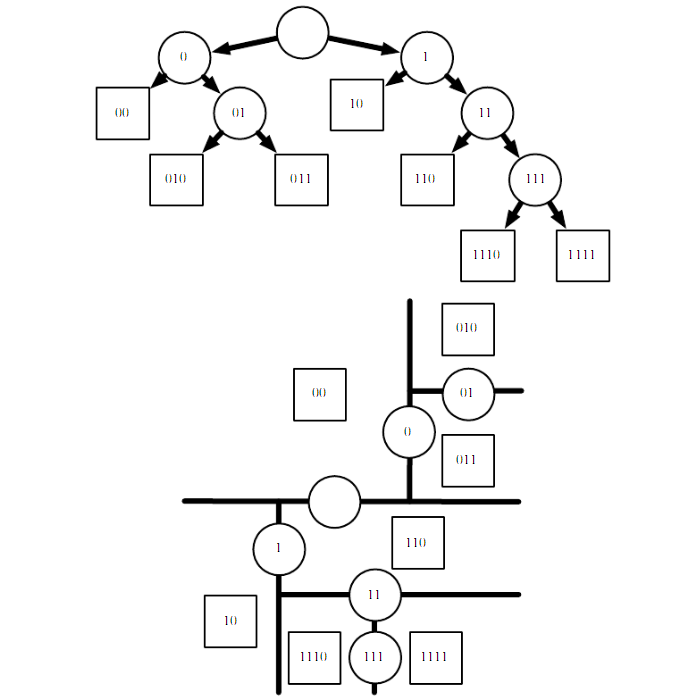
\includegraphics[width=6in]{fig/chap5/5_7.png} 
   \caption{决策树的运作机理。(上图)树的每个节点选择将输入样本送至左子节点(0)或右子节点(1)。中间节点画作圆圈,叶子节点画作方块。每个节点都以二级制字符串表示其在树中的位置,在其父节点的识别编码后增补字节(0=左或上,1=右或下)。(下图)树将输入空间划分成不同区域。这个2D平面显示了决策树如何划分$R^{2}$,中间节点画在给样本分类的分割线上,叶子节点画在样本对应区域的中心。结果是一个分段等值函数,每个叶子节点都相当于一段。每个叶子节点都需要至少一个样本才能定义,所以决策树不能学习到局部最大值比样本数量还多的函数。}
   \label{fig:5_7}
\end{figure}

另有一类学习算法也将输入孔建分成了不同的区域,并且每个域自有独立的参数,这就是\textbf{决策树}(decision tree, Breiman et al.)及其变种。如\ref{fig:5_7}所示,决策树的每个节点都对应输入空间里的不同区域,每个区域再被中间节点细分为子区域,并形成子节点(通常基于轴向切分)。空间由此继续细分为不重叠的区域,建立起叶子节点(leaf node)与输入区域(input region)之间的一一对应。每个叶子节点通常将来自同一输入区域的点映射到相同的输出。

决策树一般通过特殊的算法训练,这些算法超出了本书的范畴。如果一个学习算法可以学习任意规模的树,那么我们就可以认为该算法是无参数的,尽管在实际应用中决策树通常都经过基于规模限制的正则化(regularization)以转换为有参数模型。

决策树在使用中经常经过轴向切分(axis-aligned split),每个节点对应一个不变的输出,很多逻辑回归都能轻易解决的问题对决策树却可能很困难。例如,如果我们有一个二分类问题,当$x_{2} > x_{1}$时为正类,那么决策边界可能就不是轴向的。于是决策树就需要结合多个节点来估测决策边界,估测过程是调用一个阶跃函数(step function)在正确的决策函数边界上做等值、轴向的反复走步。

如前所述,近邻预测器和决策树存在很多限制,然而当计算资源有限的时候它们还是非常实用的。通过思考更复杂的高级算法与k近邻、决策树之间的相似与差异,我们可以获得发现更精巧算法的直觉。

关于传统监督学习算法的材料,可查看Murphy(2012), Bishop(2006), Hastie et al.(2001)或者其他机器学习课本。

\section{非监督学习算法}
\label{sec:5.8}

前承\ref{sec:5.1.3}节,无监督算法只有“特征”而没有监督信号。监督算法和非监督算法之间并没有明确严苛的区别,因为一个值属于特征还是监督者提供的标签,这本来也不存在客观定义。一般来讲,无监督学习指的是那些不借助人为干预或外部信息,直接从分布中提取信息的算法。与其高度相关的概念有:密度估计,样例提取,降噪,流形,聚类等。

有个经典的无监督学习任务,就是寻找数据的“最佳”表征。这里的“最佳”指的是尽可能多的保留$x$的信息,同时保证表征的形式比$x$本身更加简单。

定义更简单的表征可以有多种方式。三种最常见的是低维表征(low-dimensional representation)、稀疏表征(sparse representation)和独立(independent representation)表征。低维表征试图尽量压缩信息;稀疏表征(Barlow, 1989;Olshausen and Field, 1996;Hinton and Ghahramani, 1997)将数据集嵌入到另一个主要由0构成的表征里。使用稀疏表征往往要升维,整体结构是将数据分发至表征空间的各个轴上;独立表征则试图理清数据变化背后的来源,以使表征的每个维度之间都服从统计独立。

当然这三个标准并非互斥关系。低维表征常常降低元素之间的依赖性,这是因为压缩信息量的一种常用方法就是识别并剔除数据中的冗余关系。冗余的降低让降维算法可以直接忽略少部分信息以达到更大的压缩程度。

表征(representation)是深度学习的核心命题,也是本书的核心命题。在这一节中,我们开发了几个表征学习的例子,这些示例算法将展示如何实现上面所有的三个判据。之后的章节也将介绍更多从不同角度演绎这三大判据的表征学习算法以及其他判据。

\subsection{主成分分析}
\label{sec:5.8.1}

在\ref{sec:2.12}中,我们已经了解到,主成分分析(PCA, principal component analysis)算法提供了一种压缩数据的方法。我们同样把PCA看作是一种无监督学习算法,它从数据中学习表征,这样的表征基于以上提到的两种判据。PCA学习维数低于初始输入的表征,也学习一个元素与其他元素线性无关的表征。这正是统计独立表征学习的第一步。为了获得完全的独立性,表征学习算法必须将变量之间的非线性关系也识别并剔除掉。

\begin{figure}[htbp]
   \centering
   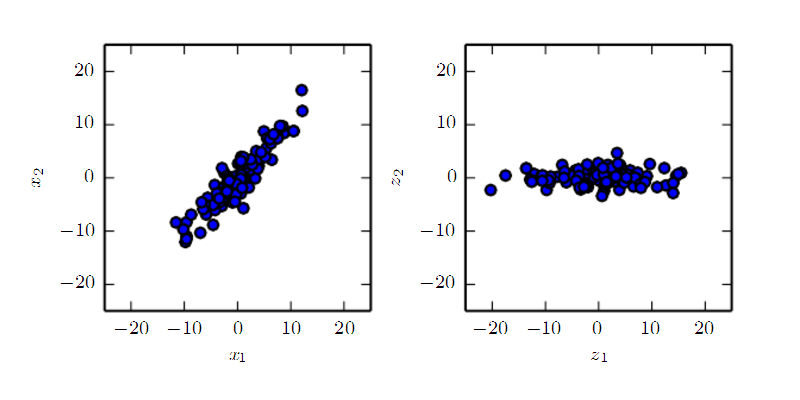
\includegraphics[width=6in]{fig/chap5/5_8.png} 
   \caption{PCA学习一种线性投影方式,使变化最大的方向与新空间的轴平行。(左图)初始数据由样本$x$构成,在这一空间中,数据的变化可能与坐标轴不平行。(右图)经过变换的数据$z=x^{T}W$现在基上是沿着轴$z_1$变化。第二大的变化方向则沿着$z_2$.}
   \label{fig:5_8}
\end{figure}

PCA学习数据的正交线性变换,将输入$x$投影到表征$z$,如\ref{fig:5_8}所示。在\ref{sec:2.12}中已经介绍过,我们可以学习构建原始数据的“最佳”一维表征(最小二乘法),这一表征其实就对应数据的第一个主成分。接着我们可以把PCA用作一种简单有效的降维方法来尽可能多的保留数据中的信息(同样根据最小二乘法)。接下来,我们将学习PCA表征如何与原始数据表征\textit{X}“去相关”。

考虑一个$m\times n$的设计矩阵$X$。假设数据的平均值为0,$E[x]=0$。如果非零,只需在预处理中将所有数据同时减去现有均值即可。

$X$的无偏协方差矩阵写作:
\begin{equation}
	Var[x] = \frac{1}{m-1}X^{T}X
   \label{form:5.85}
\end{equation}

PCA找到一个表征(通过线性变换)$z=x^{T}W$使$Var[z]$为对角阵。
在\ref{sec:2.12}中,我们已知设计矩阵$X$的主成分由$X^{T}X$的特征向量给出:
\begin{equation}
	X^{T}X = W\Lambda W^{T}
   \label{form:5.86}
\end{equation}

本节,我们将挖掘另一种主成分的推导方法。主成分也可以由奇异值分解(SVD)得到。特别地,他们就是$X$的右奇异向量。为证此理,设$W$为分解$X=U\Sigma W^{T}$的右奇异向量。再将$W$的原始特征向量还原为特征向量基。
\begin{equation}
	X^{T}X = (U\Sigma W^{T})^{T} U\Sigma W^{T} = W\Sigma^{2}W^{T}
   \label{form:5.87}
\end{equation}

SVD可以帮助我们证明PCA可以得到对角的$Var[z]$。对$X$做SVD,我们可以将$X$的方差写作:
\begin{align}
	Var[x] & = \frac{1}{m-1}X^{T}X\\
	&= \frac{1}{m-1}(U\Sigma W^T)^T U\Sigma W^T\\
	&=\frac{1}{m-1}W\Sigma ^T U^T U \Sigma W^T\\
	&=\frac{1}{m-1}W \Sigma ^2 W^T\\
\end{align}

上面的推导中我们用到了$U^T U = I$因为奇异值分解的矩阵$U$被定义为正交矩阵。下面证明如果我们取$z=x^T W$,可以确定$z$的协方差是对角矩阵:
\begin{align}
	Var[x] & = \frac{1}{m-1}Z^{T}Z\\
	&= \frac{1}{m-1}W^T X^T X W\\
	&=\frac{1}{m-1}W^T W \Sigma ^2 W W^T\\
	&=\frac{1}{m-1}\Sigma ^2\\
\end{align}
这次我们利用了$W^T W = I$,同样来自SVD的定义。

以上分析展示了当我们通过线性变换$W$将数据$x$投影到$z$的时候,所生成的表征拥有对角协方差矩阵($\Sigma ^2$),也就说明了$z$的每个元素都是相互独立的。

将数据变换成为元素相互独立的表征,这种能力是PCA的重要属性,也展现了表征的作用在于试图理清数据背后未知的变化因子。在PCA当中,这种理顺工作的形式是旋转输入空间使变化的主轴与新的表征空间$z$的基向量平行。

相关性(correlation)是数据元素之间依赖性(dependency)的重要组成部分,我们也同样对表征学习如何理顺更复杂的特征依赖感兴趣。为此,除了简单的线性变换,我们还有更多工作要做。

\subsection{k平均聚类}
\label{sec:5.8.2}

另一个简单的表征学习实例是k平均聚类(k-means clustering)。k平均算法将训练集分为k个组,每个组内部的样本相互都很接近。我们可以进一步认为该算法提供了一个k维的o独热码向量$h$来表征输入$x$。如果$x$属于一个类$i$,则$h_i=1$且$h$的其他元均为0。

k平均聚类提供的独热码正是稀疏表征的一个实例,因为每个输入的绝大多数元都是0。之后我们会接触到其他算法,它们能够学习更灵活的稀疏表征——每个输入不止有一个元为1。独热码是稀疏矩阵的极端情况,因为它丢失了分布表征的很多优点。但同时独热码也赋予了算法统计上的优势(天然地表达出同类样本相互接近)而且也带来了计算优势,整个表征可由一个整数代表。

k平均算法首先对不同的值生成k个不同的“质心”${\mu^{(1)},...,\mu^{(k)}}$,然后交替进行以下两个步骤直至收敛。步骤一:每个训练样本都被分配到某个组i当中,i就是与之最近的质心$\mu^{(i)}$的索引。步骤二:每个质心$\mu^{(i)}$更新为本组内所有训练样本$x^{(j)}$的平均值。

聚类问题的一大困难就是其天然具有病态性质,也就是并不存在一个绝对判据来衡量数据的聚类结果与真实世界多么符合。我们可以聚类的某些性质诸如分组质心到各成员的平均欧几里得距离。这可以表示我们能够在多大程度上从聚类重建原始训练数据,但是我们仍未知道聚类与真实世界的性质相去几何。

更有甚者,可能存在多种聚类结果都与真实世界的同一性质吻合良好,我们找到的可能是一个与某种性质相关、同样有效却与聚类任务本质无关的另一聚类。比如,假设我们正在一个由红色卡车、红色汽车、灰色卡车和灰色汽车组成的数据集上同时运行两个聚类算法。如果我们让两个算法各自进行二元聚类,一个算法可能按照外形分为汽车和卡车;另一算法可能按照颜色分为红色交通工具和灰色交通工具。如果再来第三个算法自动指定聚类数量,又可能分为四组——红色卡车、红色汽车、灰色卡车和灰色汽车。新算法至少同时捕捉到了两种性质的差异,但是却失去了相似性的信息。红色汽车与灰色汽车分属不同组别。聚类算法的输出并没有告诉我们,相比于灰色卡车,红色汽车与灰色汽车更接近,因为两者在颜色/外形上都不同,虽然我们都知道但算法却无法识别。

比起独热码,我们更倾向于分布表征,以上这一问题正表现出了部分原因。分布表征可以使每个交通工具具有两个性质——一个表征颜色一个表征外形(汽车/卡车)。这还未必就是最佳表征(学习算法怎么知道我们感兴趣的是颜色和外形,而非制造商和车龄呢?),但是已经减轻了算法猜测应该关照哪些属性的计算负担。并且由此我们将能够以高细粒度的方式来衡量物体之间的相似度——对比多种属性而非匹配单一属性。

\section{随机梯度下降法}
\label{sec:5.9}

\section{构建机器学习算法}
\label{sec:5.10}

\section{深度学习算法的动力}
\label{sec:5.11}
